\documentclass[a4paper]{article}
\usepackage{geometry}
\usepackage{graphicx}
\usepackage{natbib}
\usepackage{amsmath}
\usepackage{amssymb}
\usepackage{amsthm}
\usepackage{paralist}
\usepackage{epstopdf}
\usepackage{tabularx}
\usepackage{longtable}
\usepackage{multirow}
\usepackage{multicol}
\usepackage[hidelinks]{hyperref}
\usepackage{fancyvrb}
\usepackage{algorithm}
\usepackage{algorithmic}
\usepackage{float}
\usepackage{paralist}
\usepackage[svgname]{xcolor}
\usepackage{enumerate}
\usepackage{array}
\usepackage{times}
\usepackage{url}
\usepackage{fancyhdr}
\usepackage{comment}
\usepackage{environ}
\usepackage{times}
\usepackage{textcomp}
\usepackage{caption}
\usepackage{listings}


\urlstyle{rm}

\setlength\parindent{0pt} % Removes all indentation from paragraphs
\theoremstyle{definition}
\newtheorem{definition}{Definition}[]
\newtheorem{conjecture}{Conjecture}[]
\newtheorem{example}{Example}[]
\newtheorem{theorem}{Theorem}[]
\newtheorem{lemma}{Lemma}
\newtheorem{proposition}{Proposition}
\newtheorem{corollary}{Corollary}

\floatname{algorithm}{Procedure}
\renewcommand{\algorithmicrequire}{\textbf{Input:}}
\renewcommand{\algorithmicensure}{\textbf{Output:}}
\newcommand{\abs}[1]{\lvert#1\rvert}
\newcommand{\norm}[1]{\lVert#1\rVert}
\newcommand{\RR}{\mathbb{R}}
\newcommand{\CC}{\mathbb{C}}
\newcommand{\Nat}{\mathbb{N}}
\newcommand{\br}[1]{\{#1\}}
\DeclareMathOperator*{\argmin}{arg\,min}
\DeclareMathOperator*{\argmax}{arg\,max}
\renewcommand{\qedsymbol}{$\blacksquare$}

\definecolor{dkgreen}{rgb}{0,0.6,0}
\definecolor{gray}{rgb}{0.5,0.5,0.5}
\definecolor{mauve}{rgb}{0.58,0,0.82}

\newcommand{\Var}{\mathrm{Var}}
\newcommand{\Cov}{\mathrm{Cov}}

\newcommand{\vc}[1]{\boldsymbol{#1}}
\newcommand{\xv}{\vc{x}}
\newcommand{\Sigmav}{\vc{\Sigma}}
\newcommand{\alphav}{\vc{\alpha}}
\newcommand{\muv}{\vc{\mu}}

\newcommand{\red}[1]{\textcolor{red}{#1}}

\def\x{\mathbf x}
\def\y{\mathbf y}
\def\w{\mathbf w}
\def\v{\mathbf v}
\def\E{\mathbb E}
\def\V{\mathbb V}

% TO SHOW SOLUTIONS, include following (else comment out):
\newenvironment{soln}{
    \leavevmode\color{blue}\ignorespaces
}{}


\hypersetup{
%    colorlinks,
    linkcolor={red!50!black},
    citecolor={blue!50!black},
    urlcolor={blue!80!black}
}

\geometry{
  top=1in,            % <-- you want to adjust this
  inner=1in,
  outer=1in,
  bottom=1in,
  headheight=3em,       % <-- and this
  headsep=2em,          % <-- and this
  footskip=3em,
}


\pagestyle{fancyplain}
\lhead{\fancyplain{}{Homework 2}}
\rhead{\fancyplain{}{CS 760 Machine Learning}}
\cfoot{\thepage}

\title{\textsc{Homework 2}} % Title

%%% NOTE:  Replace 'NAME HERE' etc., and delete any "\red{}" wrappers (so it won't show up as red)

\author{
$>>$Sean(Xiaoyu) Sun$<<$ \\
$>>$9078202463$<<$\\
} 

\date{}

\begin{document}

\maketitle 


\textbf{Instructions:} 
Although this is a programming homework, you only need to hand in a pdf answer file.
There is no need to submit the latex source or any code.
You can choose any programming language, as long as you implement the algorithm from scratch (e.g. do not use Weka on questions 1 to 7).  

Use this latex file as a template to develop your homework.
Submit your homework on time as a single pdf file to Canvas.
Please check Piazza for updates about the homework.

\section{A Simplified Decision Tree}
You are to implement a decision-tree learner for classification.
To simplify your work, this will not be a general purpose decision tree.  Instead, your program can assume that
\begin{itemize}
\item each item has two continuous features $\x \in \RR^2$
\item the class label is binary and encoded as $y \in \{0,1\}$
\item data files are in plaintext with one labeled item per line, separated by whitespace:
$$x_{11} \quad x_{12} \quad y_1$$
$$...$$
$$x_{n1} \quad x_{n2} \quad y_n$$
\end{itemize}

Your program should implement a decision tree learner according to the following guidelines:
\begin{itemize}
\item Candidate splits $(j,c)$ for numeric features should use a threshold $c$ in feature dimension $j$ in the form of $x_{\cdot j}\ge c$.
\item $c$ should be on values of that dimension present in the training data; i.e. the threshold is on training points, not in between training points.
\item The left branch of such a split is the ``then'' branch, and the right branch is ``else''.
\item Splits should be chosen using mutual information (i.e. information gain). If there is a tie you may break it arbitrarily.
\item The stopping criteria (for making a node into a leaf) are that 
	\begin{itemize}
	\item the node is empty, or
	\item all splits have zero mutual information
	\end{itemize}
\item To simplify, whenever there is no majority class in a leaf, let it predict $y=1$.
\end{itemize}

\section{Questions}
\begin{enumerate}
\item (Our algorithm stops at pure labels) [10 pts] If a node is not empty but contains training items with the same label, why is it guaranteed to become a leaf?  Explain.

\begin{soln} According to our simplified requirement for our Decision Tree, a node becomes a leaf when having 0 info gain. When the dataset has pure label, according to the entropy formula H(y) = -$\sum_{y}^{\infty} P(y){\log_2 P(y)}$, H(y) wll always be 0, which means mutual information gain will always be 0. So every pure-label node will be a leaf. \end{soln}

\item (Our algorithm is greedy)  [10 pts] Handcraft a small training set where both classes are present but the algorithm refuses to split; instead it makes the root a leaf and stop;
Importantly, if we were to manually force a split, the algorithm will happily continue splitting the data set further and produce a deeper tree with zero training error.
You should (1) plot your training set, (2) explain why.  Hint: you don't need more than a handful of items. 
\begin{soln} 
	    \begin{figure}[H]
	        \centering
	        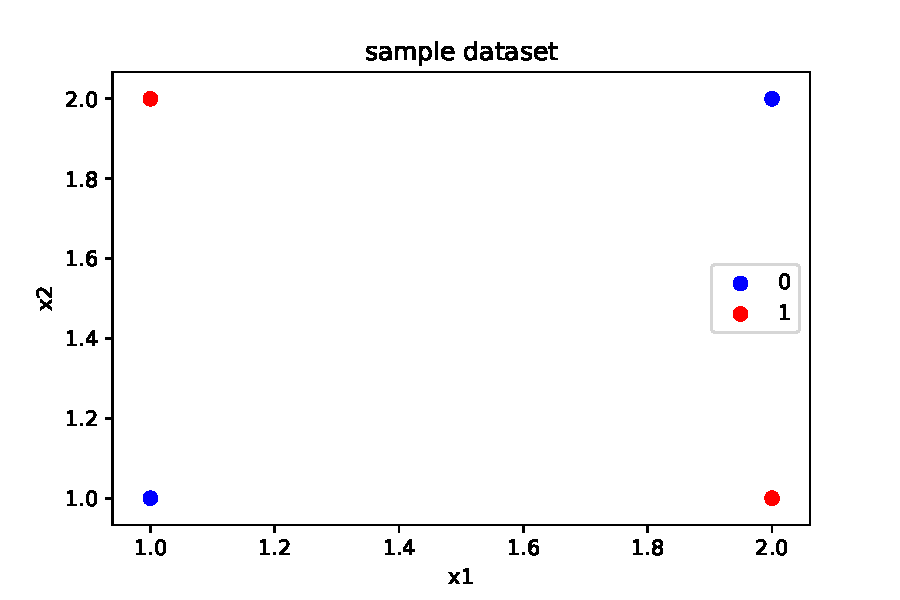
\includegraphics[width=0.6\textwidth]{question2.pdf}
	        \captionsetup{labelformat=empty}
	        \caption{}
	        \label{fig:my_label}
	    \end{figure}
In this dataset, the tree only has 4 threshold to choose (x1 = 1, x1 =2, x2 =1, x2 = 2). But each of these threshold will give 0 info gain. So the tree will stop at root node. 
However, when we manually split this dataset into 2 parts with any one of these 4 thresholds, we will get two smaller dataset having one 0-data and one 1-data. This enables the tree to further split it into two parts, each of which contains exactly one data point with label of 0 or 1, which gives 0 information gain at the end.\end{soln}

\item (Mutual information exercise)  [10 pts] Use the training set Druns.txt.  For the root node, list all candidate cuts and their mutual information.  Hint: to get $\log_2(x)$ when your programming language may be using a different base, use \verb|log(x)/log(2)|.

\begin{soln} 
	    \begin{figure}[H]
	        \centering
	        \includegraphics[width=0.3\textwidth]{question3.pdf}
	        \captionsetup{labelformat=empty}
	        \caption{}
	        \label{fig:my_label}
	    \end{figure}
\end{soln}

\item (The king of interpretability)  [10 pts] Decision tree is not the most accurate classifier in general.  However, it persists.  This is largely due to its rumored interpretability: a data scientist can easily explain a tree to a non-data scientist.  Build a tree from D3leaves.txt.  Then manually convert your tree to a set of logic rules.  Show the tree\footnote{When we say show the tree, we mean either the standard computer science tree view, or some crude plaintext representation of the tree -- as long as you explain the format.  When we say visualize the tree, we mean a plot in the 2D $\x$ space that shows how the tree will classify any points.} and the rules.

\begin{soln} 
For each data point, if it's x1 is greater than or equal to 10, it will be classified as 1. But if it's x1 is smaller than 10, we need to check its x2's value. If it's x2's value is grater than or equal to 3, it will be classified as 1 again. But if it's x2 is smaller than 3, it will be classified as 0.

The decision tree is visualized as follow: 
	    \begin{figure}[H]
	        \centering
	        \includegraphics[width=0.3\textwidth]{question4.pdf}
	        \captionsetup{labelformat=empty}
	        \caption{}
	        \label{fig:my_label}
	    \end{figure}
\end{soln}

\item (Or is it?)  [20 pts] For this question only, make sure you DO NOT VISUALIZE the data sets or plot your tree's decision boundary in the 2D $\x$ space.  If your code does that, turn it off before proceeding.  This is because you want to see your own reaction when trying to interpret a tree.  You will get points no matter what your interpretation is.
And we will ask you to visualize them in the next question anyway.
  \begin{itemize}
  \item Build a decision tree on D1.txt.  Show it to us in any format (e.g. could be a standard binary tree with nodes and arrows, and denote the rule at each leaf node; or Weka style plaintext tree; or as simple as plaintext output where each line represents a node with appropriate line number pointers to child nodes; whatever is convenient for you). Again, do not visualize the data set or the tree in the $\x$ input space.  In real tasks you will not be able to visualize the whole high dimensional input space anyway, so we don't want you to ``cheat'' here.

\begin{soln} 

Decision tree on D1.txt:

\begin{lstlisting}
x2 >= 0.201829?
Then:
  Predict  1
Else:
  Predict  0
\end{lstlisting}
\end{soln}
  \item Look at your tree in the above format (remember, you should not visualize the 2D dataset or your tree's decision boundary) and try to interpret the decision boundary in human understandable English. 

\begin{soln} 
In this decision tree, label of every data point totally depends on x2's value. When x2 is greater than or equal to 0.201829, this data point will be classified as 1; if x2 is smaller than 0.201829, it will be classified as 0
\end{soln}

  \item Build a decision tree on D2.txt.  Show it to us.
\begin{soln} 

Decision tree on D2.txt: 

\begin{lstlisting}
x1 >= 0.533076?
Then:
  |x2 >= 0.383738?
  |Then:
  |  |x1 >= 0.5503640000000001?
  |  |Then:
  |  |  |Predict  1
  |  |Else:
  |  |  |x2 >= 0.474971?
  |  |  |Then:
  |  |  |  |Predict  1
  |  |  |Else:
  |  |  |  |Predict  0
  |Else:
  |  |x1 >= 0.761423?
  |  |Then:
  |  |  |x2 >= 0.191206?
  |  |  |Then:
  |  |  |  |Predict  1
  |  |  |Else:
  |  |  |  |x1 >= 0.9048200000000001?
  |  |  |  |Then:
  |  |  |  |  |x2 >= 0.037708?
  |  |  |  |  |Then:
  |  |  |  |  |  |x1 >= 0.930371?
  |  |  |  |  |  |Then:
  |  |  |  |  |  |  |Predict  1
  |  |  |  |  |  |Else:
  |  |  |  |  |  |  |x1 >= 0.927522?
  |  |  |  |  |  |  |Then:
  |  |  |  |  |  |  |  |Predict  0
  |  |  |  |  |  |  |Else:
  |  |  |  |  |  |  |  |Predict  1
  |  |  |  |  |Else:
  |  |  |  |  |  |Predict  0
  |  |  |  |Else:
  |  |  |  |  |x2 >= 0.169053?
  |  |  |  |  |Then:
  |  |  |  |  |  |x1 >= 0.850316?
  |  |  |  |  |  |Then:
  |  |  |  |  |  |  |Predict  1
  |  |  |  |  |  |Else:
  |  |  |  |  |  |  |Predict  0
  |  |  |  |  |Else:
  |  |  |  |  |  |Predict  0
  |  |Else:
  |  |  |x2 >= 0.301105?
  |  |  |Then:
  |  |  |  |x1 >= 0.66337?
  |  |  |  |Then:
  |  |  |  |  |Predict  1
  |  |  |  |Else:
  |  |  |  |  |Predict  0
  |  |  |Else:
  |  |  |  |Predict  0
Else:
  |x2 >= 0.639018?
  |Then:
  |  |x1 >= 0.111076?
  |  |Then:
  |  |  |x2 >= 0.861?
  |  |  |Then:
  |  |  |  |Predict  1
  |  |  |Else:
  |  |  |  |x1 >= 0.33046?
  |  |  |  |Then:
  |  |  |  |  |Predict  1
  |  |  |  |Else:
  |  |  |  |  |x2 >= 0.745406?
  |  |  |  |  |Then:
  |  |  |  |  |  |x1 >= 0.25404899999999997?
  |  |  |  |  |  |Then:
  |  |  |  |  |  |  |Predict  1
  |  |  |  |  |  |Else:
  |  |  |  |  |  |  |x1 >= 0.191915?
  |  |  |  |  |  |  |Then:
  |  |  |  |  |  |  |  |x2 >= 0.792752?
  |  |  |  |  |  |  |  |Then:
  |  |  |  |  |  |  |  |  |Predict  1
  |  |  |  |  |  |  |  |Else:
  |  |  |  |  |  |  |  |  |Predict  0
  |  |  |  |  |  |  |Else:
  |  |  |  |  |  |  |  |Predict  0
  |  |  |  |  |Else:
  |  |  |  |  |  |Predict  0
  |  |Else:
  |  |  |x2 >= 0.964767?
  |  |  |Then:
  |  |  |  |Predict  1
  |  |  |Else:
  |  |  |  |Predict  0
  |Else:
  |  |x2 >= 0.534979?
  |  |Then:
  |  |  |x1 >= 0.409972?
  |  |  |Then:
  |  |  |  |x1 >= 0.426073?
  |  |  |  |Then:
  |  |  |  |  |Predict  1
  |  |  |  |Else:
  |  |  |  |  |x1 >= 0.417579?
  |  |  |  |  |Then:
  |  |  |  |  |  |Predict  0
  |  |  |  |  |Else:
  |  |  |  |  |  |Predict  1
  |  |  |Else:
  |  |  |  |Predict  0
  |  |Else:
  |  |  |Predict  0
\end{lstlisting}
\end{soln}
  \item Try to interpret your D2 decision tree.
  \end{itemize}
\begin{soln}
It will be too hard to manually interpret this tree. But one thing I noticed is that there are basically same number of 0-cases and 1-cases. So I would expect this tree to split this dataset into approxmately two even parts  
\end{soln}

\item (Hypothesis space)  [10 pts] For D1.txt and D2.txt, do the following separately:
  \begin{itemize}
  \item Produce a scatter plot of the data set.
  \item Visualize your decision tree's decision boundary (or decision region, or some other ways to clearly visualize how your decision tree will make decisions in the feature space).
  \end{itemize}
Then discuss why the size of your decision trees on D1 and D2 differ.  Relate this to the hypothesis space of our decision tree algorithm. 
\begin{soln} 
	    \begin{figure}[H]
	        \centering
	        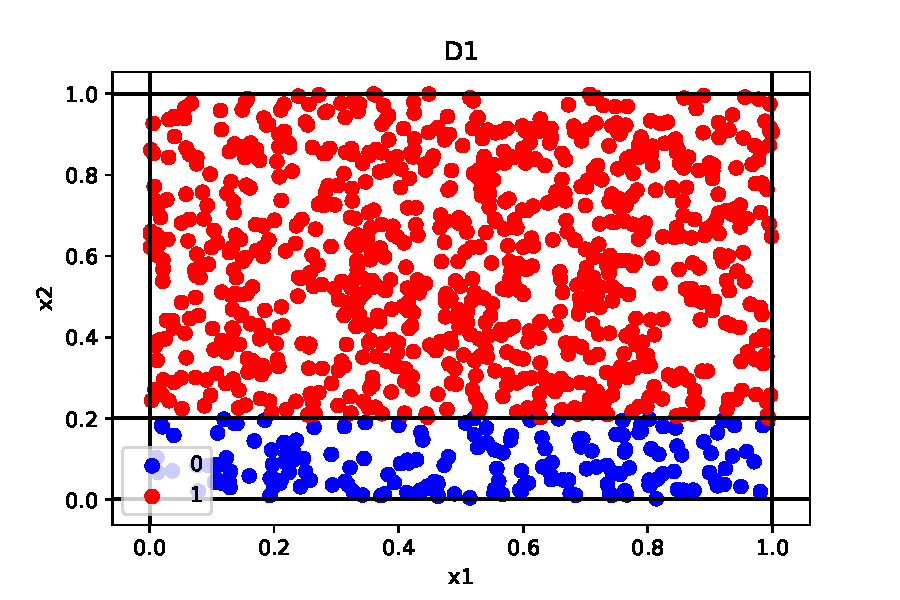
\includegraphics[width=0.4\textwidth]{question6_1.pdf}
		 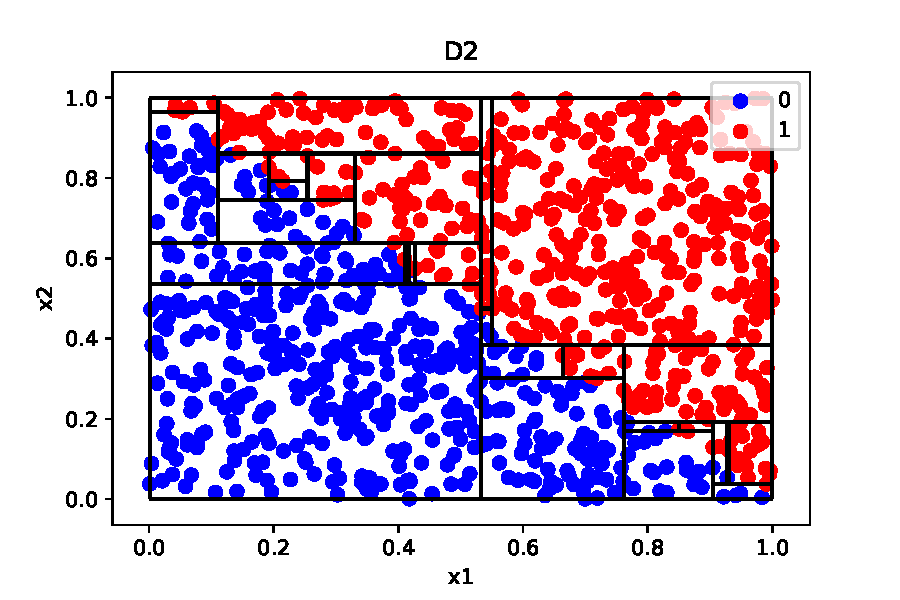
\includegraphics[width=0.4\textwidth]{question6_2.pdf}	
	        \captionsetup{labelformat=empty}
	        \caption{}
	        \label{fig:my_label}
	    \end{figure}

From the scatter plots of these two datasets, we can know that both datasets can be splitted into two decision regions by basically just one line. D1 needs a horizontal line and D2 needs a diagonal line. According to our decision tree algorithm, we can just use one feature at a time, which means our decision tree can only draw horizontal or vertical lines. So it's not hard to draw that hotizontal line for D1. However, to satisfy the diagonal in D2, we need to draw many samller horizontal or vertical lines along that diagonal line. This makes the decision tree for D2 is much bigger than the tree fro D1.

\end{soln}

\item (Learning curve)  [20 pts] We provide a data set Dbig.txt with 10000 labeled items.  Caution: Dbig.txt is sorted.
  \begin{itemize}
  \item You will randomly split Dbig.txt into a candidate training set of 8192 items and a test set (the rest).  Do this by generating a random permutation, and split at 8192.
  \item Generate a sequence of five nested training sets $D_{32} \subset D_{128} \subset D_{512} \subset D_{2048} \subset D_{8192}$ from the candidate training set.  The subscript $n$ in $D_n$ denotes training set size.  The easiest way is to take the first $n$ items from the (same) permutation above.  This sequence simulates the real world situation where you obtain more and more training data.
  \item For each $D_n$ above, train a decision tree.  Measure its test set error $err_n$.  Show three things in your answer: (1) List $n$, number of nodes in that tree, $err_n$. (2) Plot $n$ vs. $err_n$.  This is known as a learning curve (a single plot). (3) Visualize your decision trees' decision boundary (five plots).
  \end{itemize}

\begin{soln} 
Nodes numbers are:
	    \begin{figure}[H]
	        \centering
	        \includegraphics[width=0.2\textwidth]{Nodes.pdf}
	        \captionsetup{labelformat=empty}
	        \caption{}
	        \label{fig:my_label}
	    \end{figure}

Loss curve is :
	    \begin{figure}[H]
	        \centering
	        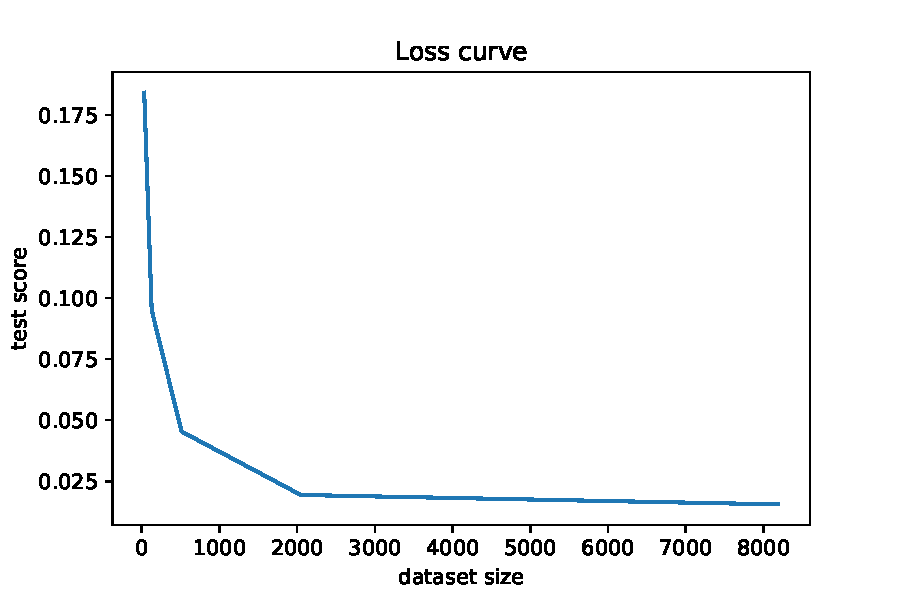
\includegraphics[width=0.4\textwidth]{loss_curve.pdf}
	        \captionsetup{labelformat=empty}
	        \caption{}
	        \label{fig:my_label}
	    \end{figure}

Boundry Visualization:
	    \begin{figure}[H]
	        \centering
	        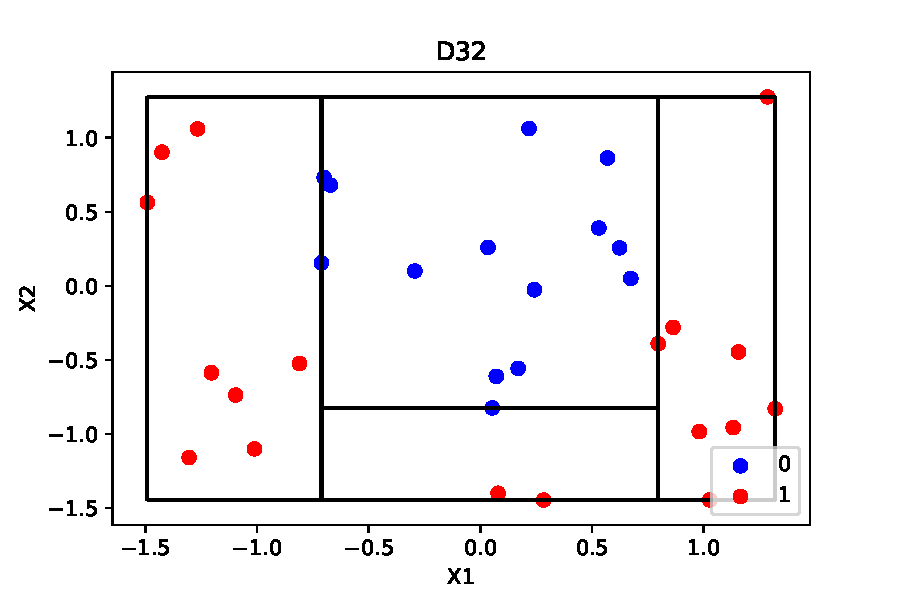
\includegraphics[width=0.4\textwidth]{question70.pdf}
	        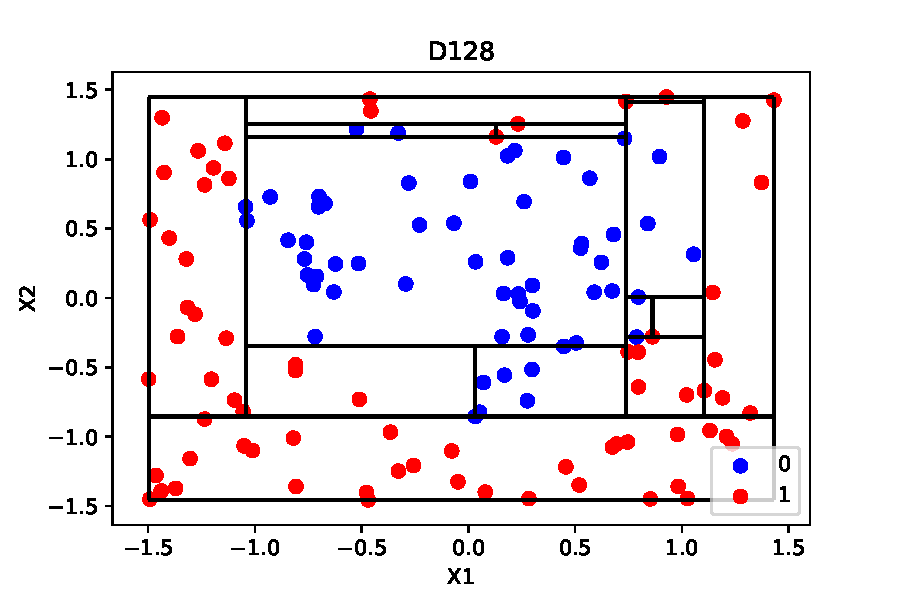
\includegraphics[width=0.4\textwidth]{question71.pdf}
	        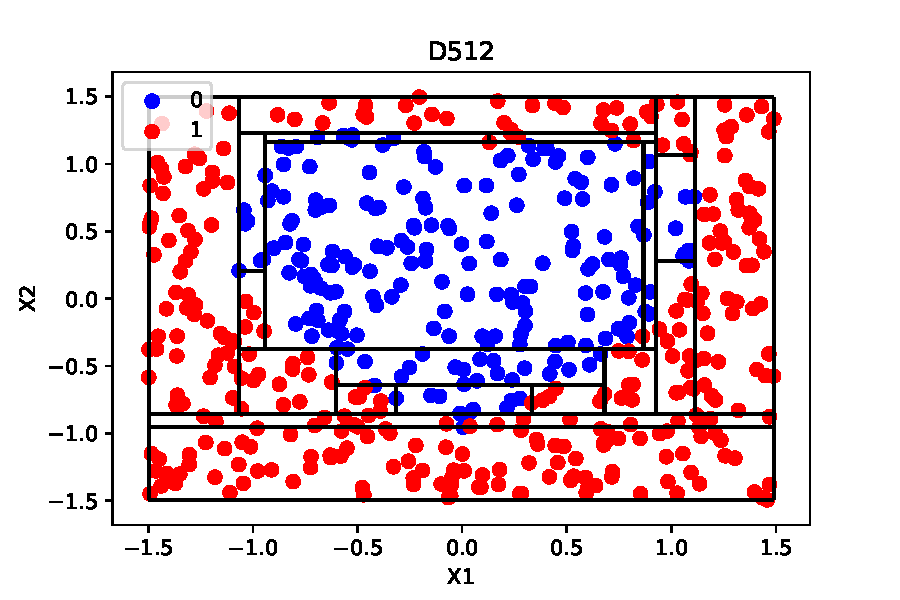
\includegraphics[width=0.4\textwidth]{question72.pdf}
	        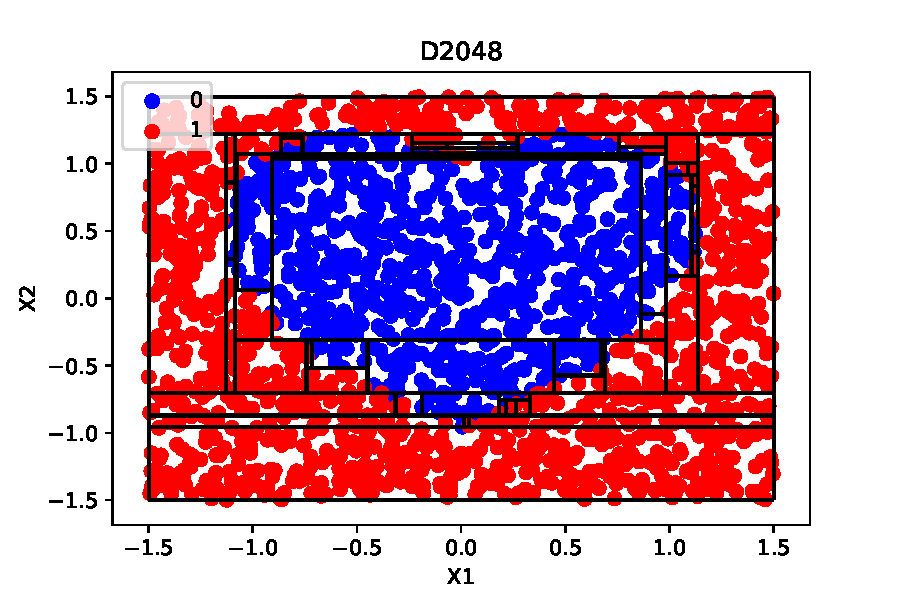
\includegraphics[width=0.4\textwidth]{question73.pdf}
	        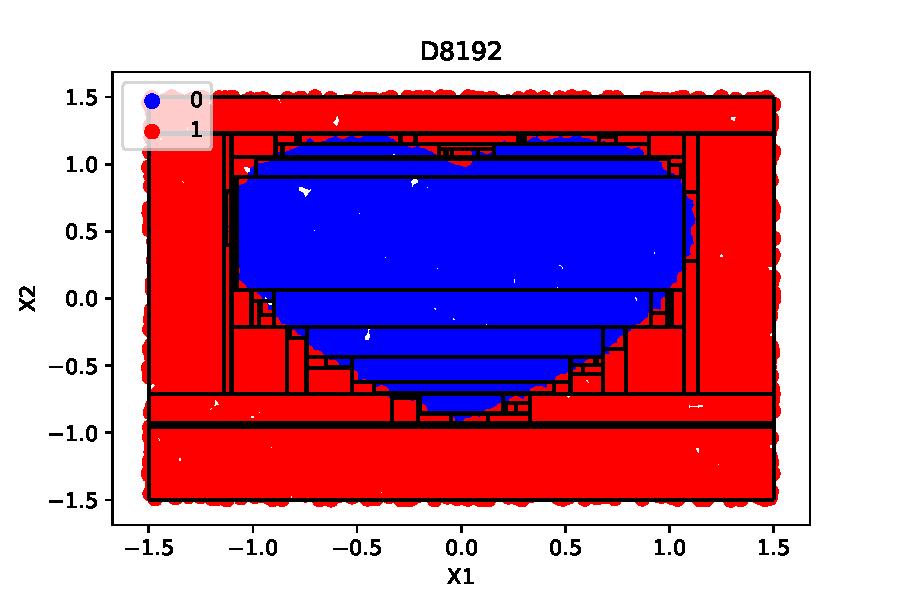
\includegraphics[width=0.4\textwidth]{question74.pdf}
	        \captionsetup{labelformat=empty}
	        \caption{}
	        \label{fig:my_label}
	    \end{figure}

\end{soln}

\end{enumerate}

\section{Weka [10 pts]}
Learn to use Weka \url{https://www.cs.waikato.ac.nz/~ml/weka/index.html}.
Convert appropriate data files into ARFF format.
Use trees/J48 as the classifier and default settings.
Produce five Weka trees for $D_{32}, D_{128} \ldots D_{8192}$.  
Show two things in your answer: (1) List $n$, number of nodes in that tree, $err_n$. (2) Plot $n$ vs. $err_n$.

\begin{soln} 
(1). N = [32, 128, 512, 2048, 8192]

(2). err = [0.21875, 0.171875, 0.058594, 0.032715, 0.015991]

(3). nodes = [7, 15, 35, 61, 133]

	    \begin{figure}[H]
	        \centering
	        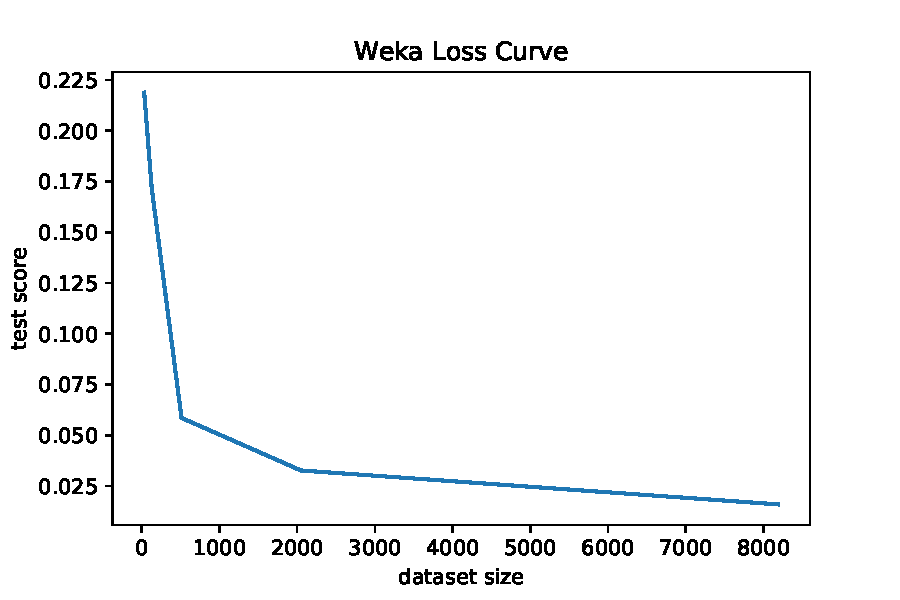
\includegraphics[width=0.4\textwidth]{Weka.pdf}
	        \captionsetup{labelformat=empty}
	        \caption{}
	        \label{fig:my_label}
	    \end{figure}
\end{soln}

\bibliographystyle{apalike}
\end{document}


